\documentclass[11pt,a4paper]{article}

\usepackage[margin=22mm,headheight=14pt]{geometry}

\usepackage{longtable,booktabs,array,hyperref,xcolor,tikz,fancyhdr}

\usepackage{fontspec,xeCJK}

\setmainfont[Ligatures=TeXOff]{Times New Roman}

\setsansfont[Ligatures=TeXOff]{Times New Roman}

\setmonofont[Ligatures=TeXOff,WordSpace={1,1,1}]{Times New Roman}

\setCJKmainfont{Noto Serif CJK SC}

\setCJKsansfont{Noto Serif CJK SC}

\setCJKmonofont{Noto Serif CJK SC}

\newfontfamily\vulcanmathsymbols{Noto Serif CJK SC}

\XeTeXgenerateactualtext=1

\definecolor{vulcan}{HTML}{BB3E23}

\pgfdeclarelayer{connections}\pgfdeclarelayer{edge labels}\pgfsetlayers{connections,main,edge labels}

\hypersetup{hidelinks}

\newcolumntype{L}[1]{>{\raggedright\arraybackslash}p{#1}}

\setlength{\emergencystretch}{5em}\tolerance=2000\hbadness=10000

\setlength{\parindent}{0pt}\setlength{\parskip}{5pt}

\pagestyle{fancy}\fancyhf{}\fancyhead[L]{\small\sffamily VULCAN}

\fancyhead[R]{\small Product design and verification}\fancyfoot[C]{\thepage}

\begin{document}

{\sffamily\huge\raggedright\textbf{RIVET-H1: Streaming SHA-256 RTL IP}\par}

{\large Technical Design and Verification Report}\par

16 October 2026 (\allowbreak{}UTC+\allowbreak{}8)\allowbreak{}\par\textcolor{vulcan}{\rule{\textwidth}{0.5pt}}

\begin{abstract}

RIVET-H1 is a synthesizable,\allowbreak{} single-clock SHA-256 core for byte-aligned messages,\allowbreak{} with a 32-bit streaming input and a backpressured 256-bit digest output. It implements FIPS 180-4 schedule expansion,\allowbreak{} 64-round compression,\allowbreak{} automatic padding,\allowbreak{} inter-block chaining and full message-length accounting. A single 64-byte buffer and iterative compressor provide a compact,\allowbreak{} serialized integration model without limiting messages to one block.


Executed Icarus verification compared 889 transactions representing 674 unique messages against Python hashlib,\allowbreak{} with zero digest mismatches,\allowbreak{} zero digest-bit mismatches and zero missing or extra outputs. All five published vectors,\allowbreak{} including one million ASCII a characters,\allowbreak{} executed through RTL. Measured compression latency was 65 cycles; sustained operation required 152 cycles per 64-byte message and 1412 cycles per 1024-byte message. Three semantic mutations were detected,\allowbreak{} and Yosys generic synthesis reported no latches. These results establish functional and generic-synthesis behavior,\allowbreak{} not physical timing,\allowbreak{} area or security certification.


\end{abstract}

\section{Architecture and design rationale}

The implementation contains exactly five functional modules,\allowbreak{} each in its same-named SystemVerilog file. The top instantiates the length,\allowbreak{} padding and compression modules; the compressor instantiates the schedule module. Gathering and compression do not overlap. This choice simplifies buffer ownership and chaining at the cost of input backpressure during every compression. The top retains one chaining state and permits only one outstanding message,\allowbreak{} including its pending digest. The diagram represents control and data dependencies,\allowbreak{} not a serial software execution pipeline. Module responsibilities and internal contracts are documented in design/\allowbreak{}ARCHITECTURE.md [\allowbreak{}E001,\allowbreak{} E003–E007]\allowbreak{}.

\begin{center}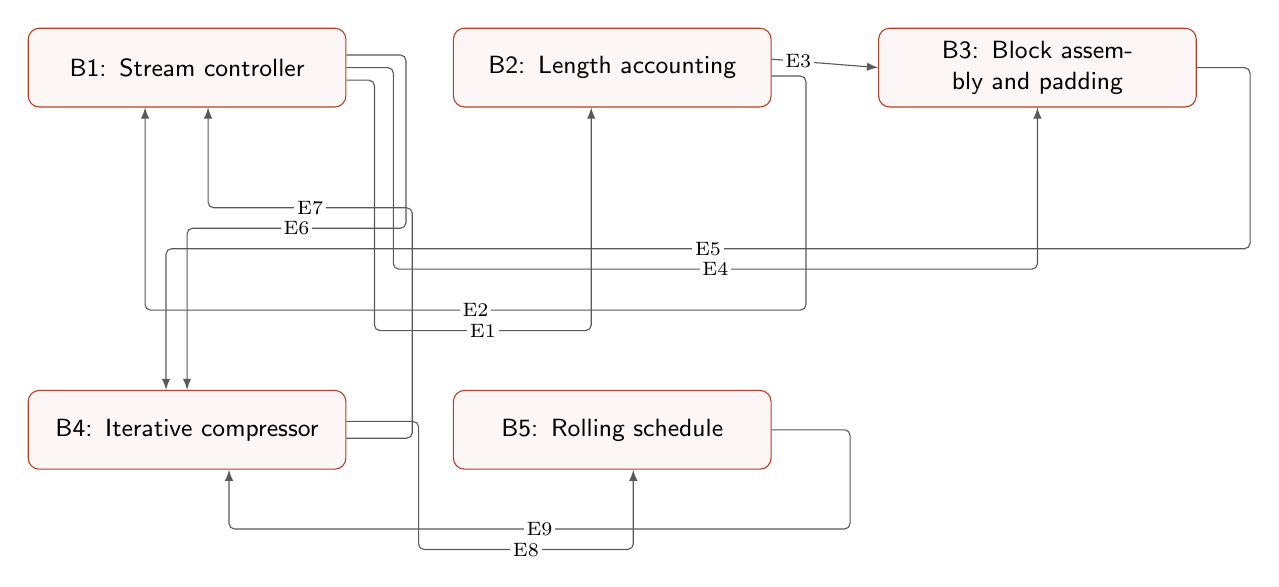
\begin{tikzpicture}[every node/.style={font=\small\sffamily},>=latex]

\node[draw=vulcan,rounded corners,fill=vulcan!4,text width=3.8cm,minimum height=1cm,align=center] (b0) at (0.0,0.0) {B1: Stream controller};

\node[draw=vulcan,rounded corners,fill=vulcan!4,text width=3.8cm,minimum height=1cm,align=center] (b1) at (5.4,0.0) {B2: Length accounting};

\node[draw=vulcan,rounded corners,fill=vulcan!4,text width=3.8cm,minimum height=1cm,align=center] (b2) at (10.8,0.0) {B3: Block assembly and padding};

\node[draw=vulcan,rounded corners,fill=vulcan!4,text width=3.8cm,minimum height=1cm,align=center] (b3) at (0.0,-4.6) {B4: Iterative compressor};

\node[draw=vulcan,rounded corners,fill=vulcan!4,text width=3.8cm,minimum height=1cm,align=center] (b4) at (5.4,-4.6) {B5: Rolling schedule};

\begin{pgfonlayer}{connections}

\draw[->,black!65,rounded corners=2pt] ([yshift=-0.160cm]b0.east) -- (2.380,-0.160) -- (2.380,-3.340) -- coordinate[midway] (e0) (5.133,-3.340) -- ([xshift=-0.267cm]b1.south);

\draw[->,black!65,rounded corners=2pt] ([yshift=-0.107cm]b1.east) -- (7.860,-0.107) -- (7.860,-3.080) -- coordinate[midway] (e1) (-0.533,-3.080) -- ([xshift=-0.533cm]b0.south);

\draw[->,black!65] ([yshift=0.107cm]b1.east) -- coordinate[pos=0.25] (e2) ([yshift=0.000cm]b2.west);

\draw[->,black!65,rounded corners=2pt] ([yshift=0.000cm]b0.east) -- (2.620,0.000) -- (2.620,-2.560) -- coordinate[midway] (e3) (10.800,-2.560) -- ([xshift=0.000cm]b2.south);

\draw[->,black!65,rounded corners=2pt] ([yshift=0.000cm]b2.east) -- (13.500,0.000) -- (13.500,-2.300) -- coordinate[midway] (e4) (-0.267,-2.300) -- ([xshift=-0.267cm]b3.north);

\draw[->,black!65,rounded corners=2pt] ([yshift=0.160cm]b0.east) -- (2.780,0.160) -- (2.780,-2.040) -- coordinate[midway] (e5) (0.000,-2.040) -- ([xshift=0.000cm]b3.north);

\draw[->,black!65,rounded corners=2pt] ([yshift=-0.107cm]b3.east) -- (2.860,-4.707) -- (2.860,-1.780) -- coordinate[midway] (e6) (0.267,-1.780) -- ([xshift=0.267cm]b0.south);

\draw[->,black!65,rounded corners=2pt] ([yshift=0.107cm]b3.east) -- (2.940,-4.493) -- (2.940,-6.120) -- coordinate[midway] (e7) (5.667,-6.120) -- ([xshift=0.267cm]b4.south);

\draw[->,black!65,rounded corners=2pt] ([yshift=0.000cm]b4.east) -- (8.420,-4.600) -- (8.420,-5.860) -- coordinate[midway] (e8) (0.533,-5.860) -- ([xshift=0.533cm]b3.south);

\end{pgfonlayer}

\begin{pgfonlayer}{edge labels}

\node[fill=white,inner sep=1pt,font=\scriptsize] at (e0) {E1};

\node[fill=white,inner sep=1pt,font=\scriptsize] at (e1) {E2};

\node[fill=white,inner sep=1pt,font=\scriptsize] at (e2) {E3};

\node[fill=white,inner sep=1pt,font=\scriptsize] at (e3) {E4};

\node[fill=white,inner sep=1pt,font=\scriptsize] at (e4) {E5};

\node[fill=white,inner sep=1pt,font=\scriptsize] at (e5) {E6};

\node[fill=white,inner sep=1pt,font=\scriptsize] at (e6) {E7};

\node[fill=white,inner sep=1pt,font=\scriptsize] at (e7) {E8};

\node[fill=white,inner sep=1pt,font=\scriptsize] at (e8) {E9};

\end{pgfonlayer}

\end{tikzpicture}\end{center}

{\small Functional block map, not a gate-level netlist. Edge identifiers match the directed relationships below. Crossings do not denote junctions; separate attachment points preserve arrow directions.}

{\small\begin{longtable}{@{}L{0.24\textwidth}L{0.7\textwidth}@{}}\toprule

\textbf{Block} & \textbf{Responsi\allowbreak{}bility}\\\midrule\endhead

B1: Stream controll\allowbreak{}er & rivet\_\allowbreak{}h1\_\allowbreak{}top validate\allowbreak{}s framing,\allowbreak{} sequence\allowbreak{}s GATHER,\allowbreak{} PREPARE,\allowbreak{} LAUNCH,\allowbreak{} WAIT\_\allowbreak{}BLOCK,\allowbreak{} OUTPUT\_\allowbreak{}DIGEST and FAULT,\allowbreak{} retains the chaining state,\allowbreak{} and reserves the complete\allowbreak{}d digest until retireme\allowbreak{}nt.\\[3pt]

B2: Length accounti\allowbreak{}ng & u\_\allowbreak{}length maintain\allowbreak{}s a 64-bit byte count. A 65-bit proposed sum detects values exceedin\allowbreak{}g 2\textasciicircum{}61-1 before an accepted beat can update the count.\\[3pt]

B3: Block assembly and padding & u\_\allowbreak{}pad owns the 512-bit block register,\allowbreak{} byte occupanc\allowbreak{}y and second-padding-block flags. It copies selected lanes,\allowbreak{} inserts padding and freezes each block during compress\allowbreak{}ion.\\[3pt]

B4: Iterativ\allowbreak{}e compress\allowbreak{}or & u\_\allowbreak{}compress captures the block and incoming chain,\allowbreak{} updates eight 32-bit working variable\allowbreak{}s over 64 rounds,\allowbreak{} then register\allowbreak{}s feed-forward results and completi\allowbreak{}on.\\[3pt]

B5: Rolling schedule & u\_\allowbreak{}schedule stores sixteen 32-bit words. It supplies W0 through W15 directly and computes W16 through W63 using the SHA-256 recurren\allowbreak{}ce,\allowbreak{} shifting the rolling window during expansio\allowbreak{}n.\\[3pt]

\bottomrule\end{longtable}}

{\small\begin{longtable}{@{}L{0.24\textwidth}L{0.7\textwidth}@{}}\toprule

\textbf{Directed relation\allowbreak{}ship} & \textbf{Meaning}\\\midrule\endhead

E1: B1 to B2 & Legal acceptan\allowbreak{}ce and retireme\allowbreak{}nt-clear controls\\[3pt]

E2: B2 to B1 & Current count and overflow proposal\\[3pt]

E3: B2 to B3 & Original bit length,\allowbreak{} shifted through top wiring\\[3pt]

E4: B1 to B3 & Accepted payload and block-manageme\allowbreak{}nt controls\\[3pt]

E5: B3 to B4 & Frozen 512-bit compress\allowbreak{}ion block\\[3pt]

E6: B1 to B4 & Launch and incoming chaining state\\[3pt]

E7: B4 to B1 & Completi\allowbreak{}on and feed-forward chaining result\\[3pt]

E8: B4 to B5 & Block load,\allowbreak{} round index and schedule step\\[3pt]

E9: B5 to B4 & Current 32-bit schedule word\\[3pt]

\bottomrule\end{longtable}}

\section{Interfaces and configuration}

{\small\begin{longtable}{@{}L{0.2\textwidth}L{0.12\textwidth}L{0.1\textwidth}L{0.48\textwidth}@{}}\toprule

\textbf{Signal /\allowbreak{} group} & \textbf{Directio\allowbreak{}n} & \textbf{Width} & \textbf{Contract}\\\midrule\endhead

clk & Input & 1 bit & Rising-edge clock for all transfer\allowbreak{}s and sequenti\allowbreak{}al state.\\[3pt]

rst\_\allowbreak{}n & Input & 1 bit & Asynchro\allowbreak{}nous active-low reset. Assertio\allowbreak{}n cancels all work and forces s\_\allowbreak{}ready,\allowbreak{} m\_\allowbreak{}valid,\allowbreak{} m\_\allowbreak{}digest and error to zero. Reset release requires external recovery/\allowbreak{}removal discipli\allowbreak{}ne.\\[3pt]

s\_\allowbreak{}valid /\allowbreak{} s\_\allowbreak{}ready & Input /\allowbreak{} output & 1 bit each & Input acceptan\allowbreak{}ce occurs only on a rising edge with rst\_\allowbreak{}n,\allowbreak{} s\_\allowbreak{}valid and s\_\allowbreak{}ready high. The producer must hold valid,\allowbreak{} data,\allowbreak{} keep and last stable while stalled.\\[3pt]

s\_\allowbreak{}data & Input & 32 bits & Unsigned packed bytes: bits 31:24 arrive first,\allowbreak{} then 23:16,\allowbreak{} 15:8 and 7:0. Unselect\allowbreak{}ed final lanes are ignored.\\[3pt]

s\_\allowbreak{}keep /\allowbreak{} s\_\allowbreak{}last & Input & 4 bits /\allowbreak{} 1 bit & Nonfinal beats require keep=\allowbreak{}1111. Final masks 1000,\allowbreak{} 1100,\allowbreak{} 1110 and 1111 select one through four bytes. An empty message uses one final beat with keep=\allowbreak{}0000; zero-byte terminat\allowbreak{}ion after prior data is illegal.\\[3pt]

m\_\allowbreak{}valid /\allowbreak{} m\_\allowbreak{}ready & Output /\allowbreak{} input & 1 bit each & Digest retireme\allowbreak{}nt occurs on a rising edge with rst\_\allowbreak{}n,\allowbreak{} m\_\allowbreak{}valid and m\_\allowbreak{}ready high. Valid and digest remain stable under backpres\allowbreak{}sure. No new input is accepted on the retireme\allowbreak{}nt edge.\\[3pt]

m\_\allowbreak{}digest & Output & 256 bits & Standard SHA-256 order: H0 occupies bits 255:224 through H7 in bits 31:0. Zero during reset; it may retain the previous digest while invalid.\\[3pt]

error & Output & 1 bit & Sticky indicati\allowbreak{}on of accepted illegal framing or length overflow. The aborted message produces no digest; input and output valid remain disabled until reset.\\[3pt]

\bottomrule\end{longtable}}

{\small\begin{longtable}{@{}L{0.23\textwidth}L{0.12\textwidth}L{0.57\textwidth}@{}}\toprule

\textbf{Paramete\allowbreak{}r} & \textbf{Default} & \textbf{Meaning /\allowbreak{} supporte\allowbreak{}d values}\\\midrule\endhead

User paramete\allowbreak{}rs & None & Only the fixed 32-bit input,\allowbreak{} 256-bit output,\allowbreak{} one-buffer configur\allowbreak{}ation is supporte\allowbreak{}d. There are no configur\allowbreak{}ation register\allowbreak{}s,\allowbreak{} initiali\allowbreak{}zation files,\allowbreak{} debug ports or paramete\allowbreak{}r variants.\\[3pt]

\bottomrule\end{longtable}}

\section{Behavior and corner cases}

\subsection{Message framing and reservation}

There is no first-message marker. The first accepted beat after reset or digest retirement begins the next message. Multiple-of-four lengths terminate with a full final beat,\allowbreak{} not an extra empty token. Input may pause indefinitely. Compression and pending output both block further acceptance; readiness returns after retirement for acceptance on the following edge [\allowbreak{}E002,\allowbreak{} E007]\allowbreak{}.

\subsection{Numerical rules and length bounds}

All SHA-256 words are unsigned 32-bit values,\allowbreak{} with additions modulo 2\textasciicircum{}32. The standard initial state,\allowbreak{} 64 constants,\allowbreak{} Ch,\allowbreak{} Maj and sigma functions are implemented. Supported message lengths are 0 through 2\textasciicircum{}61-1 bytes inclusive. Only accepted legal payload bytes increment the count; padding is excluded. Padding encodes byte\_\allowbreak{}count shifted left three as a 64-bit big-endian bit length. A widened addition detects overflow before commitment [\allowbreak{}E002–E007]\allowbreak{}.

\subsection{Schedule and chaining}

Expansion computes Wt=\allowbreak{}sigma1(\allowbreak{}Wt-2)\allowbreak{}+\allowbreak{}Wt-7+\allowbreak{}sigma0(\allowbreak{}Wt-15)\allowbreak{}+\allowbreak{}Wt-16 modulo 2\textasciicircum{}32. Small-sigma rotation/\allowbreak{}shift triples are (\allowbreak{}7,\allowbreak{}18,\allowbreak{}3)\allowbreak{} and (\allowbreak{}17,\allowbreak{}19,\allowbreak{}10)\allowbreak{}; big-sigma rotation triples are (\allowbreak{}2,\allowbreak{}13,\allowbreak{}22)\allowbreak{} and (\allowbreak{}6,\allowbreak{}11,\allowbreak{}25)\allowbreak{}. Each compression feeds its result into the next block. Digest retirement restores the standard initial state for the next message [\allowbreak{}E003,\allowbreak{} E006,\allowbreak{} E007]\allowbreak{}.

\subsection{Automatic padding}

Padding appends 0x80,\allowbreak{} zeros and the original 64-bit length. A final occupied block containing 0–55 payload bytes needs one compression; 56–63 bytes need two. A full final data block also needs a separate padding block. For message length n,\allowbreak{} total compressions equal ceil(\allowbreak{}(\allowbreak{}n+\allowbreak{}9)\allowbreak{}/\allowbreak{}64)\allowbreak{}. The 65-byte case therefore has two total blocks but only one compression remaining after its final beat [\allowbreak{}E002,\allowbreak{} E005]\allowbreak{}.

\subsection{Edge-level timing}

Handshakes sample pre-edge signals; registered results are observed post-edge. For a full-block or final-beat acceptance at E,\allowbreak{} E+\allowbreak{}1 prepares the block and E+\allowbreak{}2 launches compression. E+\allowbreak{}3 through E+\allowbreak{}66 execute rounds 0–63; E+\allowbreak{}67 registers completion; E+\allowbreak{}68 consumes it. Gathering resumes then for a nonfinal block,\allowbreak{} or digest valid appears for one-compression finalization. Two-compression finalization prepares its second block at E+\allowbreak{}68,\allowbreak{} launches at E+\allowbreak{}69,\allowbreak{} executes rounds at E+\allowbreak{}70 through E+\allowbreak{}133,\allowbreak{} registers completion at E+\allowbreak{}134 and asserts digest valid at E+\allowbreak{}135. Earliest output handshakes are E+\allowbreak{}69 and E+\allowbreak{}136 respectively [\allowbreak{}E002,\allowbreak{} E015]\allowbreak{}.

\subsection{Reset and fault priority}

Reset dominates every handshake and error condition,\allowbreak{} cancelling partial input,\allowbreak{} preparation,\allowbreak{} active rounds,\allowbreak{} pending completion and stalled output. Accepted illegal masks,\allowbreak{} nonempty zero-byte termination and overflow enter sticky FAULT. Illegal values while invalid or stalled do not themselves cause errors. Valid digests must contain no X/\allowbreak{}Z bits [\allowbreak{}E002,\allowbreak{} E007,\allowbreak{} E015]\allowbreak{}.

\section{Verification methods and measured results}

\subsection{Cryptographic correctness and coverage}

\textbf{Method.} Icarus 12.0 compilation and simulation with Python 3.12.3 hashlib comparisons. The matrix contained five published vectors,\allowbreak{} 24 specified boundary lengths,\allowbreak{} all 256 one-byte messages,\allowbreak{} eight long binary messages,\allowbreak{} 384 seeded random transactions,\allowbreak{} 200 sustained transactions and 12 traffic/\allowbreak{}gap cases.

\textbf{Result.} 889 transactions,\allowbreak{} 674 unique messages; zero digest mismatches,\allowbreak{} zero digest-bit mismatches and zero missing/\allowbreak{}extra outputs. Seeds 11,\allowbreak{} 29 and 89 each contributed 128 random messages across 0–4096 bytes and covered all 64 length residues. Long binary lengths were 4097,\allowbreak{} 8191,\allowbreak{} 8192,\allowbreak{} 8193,\allowbreak{} 16384,\allowbreak{} 32768,\allowbreak{} 65535 and 65536 bytes. Replays are not counted as new unique messages.

{\small Evidence: E008,\allowbreak{} E010,\allowbreak{} E015}

\subsection{Published vectors and independent internal reference}

\textbf{Method.} An independently authored FIPS Python model was checked against published expected digests and hashlib. Observed RTL padded blocks,\allowbreak{} schedule words and incoming/\allowbreak{}outgoing chaining states were compared with model expectations.

\textbf{Result.} All five published vectors executed: empty,\allowbreak{} abc,\allowbreak{} the standard 56-byte and 112-byte messages,\allowbreak{} and one million ASCII a characters. Detailed comparisons covered 114 blocks,\allowbreak{} including padding boundaries and long-message chaining. The million-byte vector executed 15,\allowbreak{}626 blocks and 1,\allowbreak{}000,\allowbreak{}064 rounds.

{\small Evidence: E009,\allowbreak{} E010,\allowbreak{} E015}

\subsection{Protocol,\allowbreak{} cancellation and length arithmetic}

\textbf{Method.} Directed and seeded traffic exercised legal masks,\allowbreak{} ignored lanes,\allowbreak{} gaps,\allowbreak{} output-ready transitions,\allowbreak{} stable reservations and reset recovery. Separate state-seeded length experiments checked arithmetic around 2\textasciicircum{}32 bits,\allowbreak{} 2\textasciicircum{}32 bytes and the maximum supported count.

\textbf{Result.} 31 sticky-fault/\allowbreak{}recovery cases,\allowbreak{} ten reset-cancellation phases,\allowbreak{} three reset-priority cases and 258 stalled cycles with continuous next-message valid passed. Eleven traffic replays each held the digest for 256 extra cycles. All 135 arithmetic comparisons passed,\allowbreak{} including exact-maximum acceptance and overflow by one through four bytes. The run recorded 936 output handshakes including recovery traffic,\allowbreak{} distinct from the 889 matrix transactions.

{\small Evidence: E008,\allowbreak{} E010,\allowbreak{} E015}

\subsection{Exact compression and finalization cycles}

\textbf{Method.} Cycle monitors checked launch,\allowbreak{} every round index,\allowbreak{} registered completion,\allowbreak{} first-valid and retirement edges. The retained transaction ledger records latency,\allowbreak{} blocks,\allowbreak{} rounds and stalls.

\textbf{Result.} Every completed block obeyed 64 round-update edges and 65 launch-to-completion cycles. Final-beat latency was exactly 68 or 135 cycles. First-input-to-valid latency for 55/\allowbreak{}56/\allowbreak{}63/\allowbreak{}64/\allowbreak{}65-byte boundary inputs was 81/\allowbreak{}148/\allowbreak{}150/\allowbreak{}150/\allowbreak{}152 cycles. The complete behavior run elapsed 3,\allowbreak{}086,\allowbreak{}069 cycles; its 33,\allowbreak{}324 launches and 2,\allowbreak{}132,\allowbreak{}577 round edges include protocol and cancelled work.

{\small Evidence: E002,\allowbreak{} E008,\allowbreak{} E015}

\subsection{Sustained payload throughput}

\textbf{Method.} Two runs each sent 100 consecutive messages without external input gaps or output stalls. Measurement spans the first accepted input edge through the last output handshake,\allowbreak{} inclusive; padding is excluded from payload.

\textbf{Result.} 64-byte messages: 6400 payload bytes in 15,\allowbreak{}200 cycles,\allowbreak{} 152 cycles/\allowbreak{}message and 0.421052632 bytes/\allowbreak{}cycle. 1024-byte messages: 102,\allowbreak{}400 bytes in 141,\allowbreak{}200 cycles,\allowbreak{} 1412 cycles/\allowbreak{}message and 0.725212465 bytes/\allowbreak{}cycle. Individual first-input-to-valid latencies were 150 and 1410 cycles. Short messages incur proportionally greater padding overhead; both runs retain serialized compression cost.

{\small Evidence: E010,\allowbreak{} E015}

\subsection{Checker sensitivity to semantic defects}

\textbf{Method.} Three disposable RTL copies independently corrupted encoded length,\allowbreak{} changed an active schedule rotation,\allowbreak{} or substituted the initial state for inter-block chaining. Each compiled and executed against the same digest oracle,\allowbreak{} with a pristine control.

\textbf{Result.} All three mutants produced actual digest mismatches: abc exposed the length defect with 136 differing bits; a 55-byte witness exposed the rotation defect with 125; a 65-byte witness exposed the chaining defect with 136. All three controls had zero mismatches. Source hashes,\allowbreak{} mutation diffs and failing observations were retained; delivered RTL was unchanged.

{\small Evidence: E010,\allowbreak{} E016}

\subsection{Synthesizability and substantive structure}

\textbf{Method.} Yosys 0.33 executed SystemVerilog reading,\allowbreak{} hierarchy checks,\allowbreak{} process and memory lowering,\allowbreak{} optimization,\allowbreak{} generic synthesis and check -assert. Netlists were inspected before and after synthesis.

\textbf{Result.} The required five-module hierarchy and sequential state were present. No latches or unresolved blackboxes were found; consistency checks passed. Before generic synthesis there were 409 cell entries and 39 sequential cells. Afterwards there were 25,\allowbreak{}503 entries across module definitions,\allowbreak{} including four hierarchy instances,\allowbreak{} and 2391 sequential cells. These are generic resources,\allowbreak{} not physical area.

{\small Evidence: E010,\allowbreak{} E017}

\subsection{Source inventory and portable reproduction}

\textbf{Method.} Source-bound inventories measured delivered files. A fresh directory copied only five RTL files,\allowbreak{} three Python verification files and the two design documents,\allowbreak{} then executed a real child smoke suite with fresh generated outputs.

\textbf{Result.} RTL totals: five modules,\allowbreak{} 409 lines and 15,\allowbreak{}778 bytes. Module line/\allowbreak{}byte counts are top 131/\allowbreak{}4992,\allowbreak{} length 24/\allowbreak{}776,\allowbreak{} pad 61/\allowbreak{}2164,\allowbreak{} compressor 159/\allowbreak{}6581 and schedule 34/\allowbreak{}1265. Verification totals: 1079 lines and 46,\allowbreak{}152 bytes. Portable smoke passed 20 transactions representing 13 unique messages with zero mismatches or missing/\allowbreak{}extra outputs,\allowbreak{} plus protocol/\allowbreak{}reset checks and 135 arithmetic comparisons. This was bounded reproduction,\allowbreak{} not a full-matrix replay.

{\small Evidence: E003,\allowbreak{} E004,\allowbreak{} E005,\allowbreak{} E006,\allowbreak{} E007,\allowbreak{} E015,\allowbreak{} E018}

\section{Integration and use}

Use design/\allowbreak{}SPEC.md for the external contract and design/\allowbreak{}ARCHITECTURE.md for internal ownership and integration. Compile all five rtl/\allowbreak{}*\allowbreak{}.sv files and select rivet\_\allowbreak{}h1\_\allowbreak{}top; no generated source or initialization data is needed.


Static elaboration command from the project root: \texttt{iverilog -g2012 -s rivet\_\allowbreak{}h1\_\allowbreak{}top -t null rtl/\allowbreak{}rivet\_\allowbreak{}h1\_\allowbreak{}top.sv rtl/\allowbreak{}rivet\_\allowbreak{}h1\_\allowbreak{}length.sv rtl/\allowbreak{}rivet\_\allowbreak{}h1\_\allowbreak{}pad.sv rtl/\allowbreak{}rivet\_\allowbreak{}h1\_\allowbreak{}compress.sv rtl/\allowbreak{}rivet\_\allowbreak{}h1\_\allowbreak{}schedule.sv}.


Assert reset before use and synchronize its release externally as required by the target technology. Send MSB-first legal beats,\allowbreak{} preserving the complete beat during stalls. Retire the digest with m\_\allowbreak{}ready; reset after error before attempting another message.


Reproduction dependencies are Python 3 with standard-library hashlib,\allowbreak{} iverilog,\allowbreak{} vvp and yosys. No third-party Python package is required. Full behavior command: \texttt{python3 tests/\allowbreak{}verify.py --suite behavior --out evidence/\allowbreak{}behavior}. Omitting --seed runs all three required seeds.


Additional exact commands are \texttt{python3 tests/\allowbreak{}verify.py --suite sensitivity --out evidence/\allowbreak{}sensitivity},\allowbreak{} \texttt{python3 tests/\allowbreak{}verify.py --suite synthesis --out evidence/\allowbreak{}synthesis},\allowbreak{} and \texttt{python3 tests/\allowbreak{}verify.py --suite portable --out evidence/\allowbreak{}portable}. For bounded local coverage use \texttt{python3 tests/\allowbreak{}verify.py --suite smoke --out evidence/\allowbreak{}smoke}.


Each suite retains timestamped results,\allowbreak{} source hashes,\allowbreak{} tool versions,\allowbreak{} execution receipts and raw child streams beneath its output directory. The behavior result contains the complete transaction ledger. Portable reproduction copies only declared sources; prior generated testbenches,\allowbreak{} simulator images,\allowbreak{} synthesis outputs and the product report are not required inputs.


\section{Limitations and acceptance boundary}

The supported 0–2\textasciicircum{}61-1-byte range is an arithmetic and interface contract. Near-limit state-seeded experiments are not end-to-end hashing of messages approaching that bound; the largest executed published message contained one million bytes.


The design supports byte-aligned SHA-256 only,\allowbreak{} one clock,\allowbreak{} one block buffer and one outstanding message. It provides neither compression/\allowbreak{}input overlap nor simultaneous digest retirement and next-message acceptance.


Verification establishes the executed matrices and structural checks,\allowbreak{} not exhaustive formal correctness. Mutation detection demonstrates sensitivity to the three tested defects,\allowbreak{} not every possible implementation fault.


Generic synthesis does not establish technology-mapped area,\allowbreak{} maximum frequency,\allowbreak{} timing closure,\allowbreak{} power,\allowbreak{} FPGA performance or silicon-security properties. No physical implementation measurements or cryptographic certification are claimed.


\appendix\section{Source inventory}

Production inventory: 5 Verilog/\allowbreak{}SystemVerilog files; 398 nonblank,\allowbreak{} non-comment lines. Source size is not a correctness or quality metric.

{\small\begin{longtable}{@{}L{0.61\textwidth}L{0.15\textwidth}L{0.15\textwidth}@{}}\toprule

\textbf{Producti\allowbreak{}on file} & \textbf{Physical lines} & \textbf{Code lines}\\\midrule\endhead

rtl/\allowbreak{}rivet\_\allowbreak{}h1\_\allowbreak{}compress.sv & 159 & 155\\[3pt]

rtl/\allowbreak{}rivet\_\allowbreak{}h1\_\allowbreak{}length.sv & 24 & 23\\[3pt]

rtl/\allowbreak{}rivet\_\allowbreak{}h1\_\allowbreak{}pad.sv & 61 & 60\\[3pt]

rtl/\allowbreak{}rivet\_\allowbreak{}h1\_\allowbreak{}schedule.sv & 34 & 33\\[3pt]

rtl/\allowbreak{}rivet\_\allowbreak{}h1\_\allowbreak{}top.sv & 131 & 127\\[3pt]

\bottomrule\end{longtable}}

\section{Verification record index}

{\small\begin{longtable}{@{}L{0.57\textwidth}L{0.16\textwidth}L{0.17\textwidth}@{}}\toprule

\textbf{Recorded check} & \textbf{Outcome} & \textbf{Executio\allowbreak{}n time (\allowbreak{}s)\allowbreak{}}\\\midrule\endhead

behavior & passed & 146.500\\[3pt]

sensitiv\allowbreak{}ity & passed & 0.729\\[3pt]

synthesi\allowbreak{}s & passed & 34.968\\[3pt]

portable & passed & 1.330\\[3pt]

\bottomrule\end{longtable}}

Execution times include tool and provider waiting; they are not hardware latency or model utilization.

{\small\begin{longtable}{@{}L{0.12\textwidth}L{0.82\textwidth}@{}}\toprule

\textbf{Referenc\allowbreak{}e} & \textbf{Original project-relative record}\\\midrule\endhead

E002 & design/\allowbreak{}SPEC.md\\[3pt]

E003 & rtl/\allowbreak{}rivet\_\allowbreak{}h1\_\allowbreak{}compress.sv\\[3pt]

E004 & rtl/\allowbreak{}rivet\_\allowbreak{}h1\_\allowbreak{}length.sv\\[3pt]

E005 & rtl/\allowbreak{}rivet\_\allowbreak{}h1\_\allowbreak{}pad.sv\\[3pt]

E006 & rtl/\allowbreak{}rivet\_\allowbreak{}h1\_\allowbreak{}schedule.sv\\[3pt]

E007 & rtl/\allowbreak{}rivet\_\allowbreak{}h1\_\allowbreak{}top.sv\\[3pt]

E008 & tests/\allowbreak{}bench.py\\[3pt]

E009 & tests/\allowbreak{}model.py\\[3pt]

E010 & tests/\allowbreak{}verify.py\\[3pt]

E015 & .vulcan/\allowbreak{}engineer\allowbreak{}ing/\allowbreak{}run-0001/\allowbreak{}attempt-0003/\allowbreak{}stdout.log\\[3pt]

E016 & .vulcan/\allowbreak{}engineer\allowbreak{}ing/\allowbreak{}run-0001/\allowbreak{}attempt-0004/\allowbreak{}stdout.log\\[3pt]

E017 & .vulcan/\allowbreak{}engineer\allowbreak{}ing/\allowbreak{}run-0001/\allowbreak{}attempt-0005/\allowbreak{}stdout.log\\[3pt]

E018 & .vulcan/\allowbreak{}engineer\allowbreak{}ing/\allowbreak{}run-0001/\allowbreak{}attempt-0006/\allowbreak{}stdout.log\\[3pt]

\bottomrule\end{longtable}}

\section{Document provenance}

Engineering was independently accepted for the recorded source and evidence identity. This is not exhaustive proof, hardware deployment or physical signoff. The companion REPORT.md records the exact report approval and source manifest, and links the English/Chinese journeys containing original failures and interventions. A report number identifies a generation attempt, not a new hardware revision.

No developer attribution was supplied; none has been inferred.

\end{document}
